% This is "sig-alternate.tex" V2.1 April 2013
% This file should be compiled with V2.5 of "sig-alternate.cls" May 2012
%
% This example file demonstrates the use of the 'sig-alternate.cls'
% V2.5 LaTeX2e document class file. It is for those submitting
% articles to ACM Conference Proceedings WHO DO NOT WISH TO
% STRICTLY ADHERE TO THE SIGS (PUBS-BOARD-ENDORSED) STYLE.
% The 'sig-alternate.cls' file will produce a similar-looking,
% albeit, 'tighter' paper resulting in, invariably, fewer pages.
%
% ----------------------------------------------------------------------------------------------------------------
% This .tex file (and associated .cls V2.5) produces:
%       1) The Permission Statement
%       2) The Conference (location) Info information
%       3) The Copyright Line with ACM data
%       4) NO page numbers
%
% as against the acm_proc_article-sp.cls file which
% DOES NOT produce 1) thru' 3) above.
%
% Using 'sig-alternate.cls' you have control, however, from within
% the source .tex file, over both the CopyrightYear
% (defaulted to 200X) and the ACM Copyright Data
% (defaulted to X-XXXXX-XX-X/XX/XX).
% e.g.
% \CopyrightYear{2007} will cause 2007 to appear in the copyright line.
% \crdata{0-12345-67-8/90/12} will cause 0-12345-67-8/90/12 to appear in the copyright line.
%
% ---------------------------------------------------------------------------------------------------------------
% This .tex source is an example which *does* use
% the .bib file (from which the .bbl file % is produced).
% REMEMBER HOWEVER: After having produced the .bbl file,
% and prior to final submission, you *NEED* to 'insert'
% your .bbl file into your source .tex file so as to provide
% ONE 'self-contained' source file.
%
% ================= IF YOU HAVE QUESTIONS =======================
% Questions regarding the SIGS styles, SIGS policies and
% procedures, Conferences etc. should be sent to
% Adrienne Griscti (griscti@acm.org)
%
% Technical questions _only_ to
% Gerald Murray (murray@hq.acm.org)
% ===============================================================
%
% For tracking purposes - this is V2.0 - May 2012

\documentclass{sig-alternate-05-2015}

\usepackage{epstopdf}
\usepackage{float}
\usepackage{graphicx}
\usepackage{amsmath}
\usepackage[caption=false,font=footnotesize]{subfig}
\usepackage{textcomp}

\begin{document}

% Copyright
%\setcopyright{acmcopyright}
%\setcopyright{acmlicensed}
%\setcopyright{rightsretained}
%\setcopyright{usgov}
%\setcopyright{usgovmixed}
%\setcopyright{cagov}
%\setcopyright{cagovmixed}


% DOI
%\doi{10.475/123_4}

% ISBN
%\isbn{123-4567-24-567/08/06}

%Conference
%\conferenceinfo{PLDI '13}{June 16--19, 2013, Seattle, WA, USA}

%\acmPrice{\$15.00}

%
% --- Author Metadata here ---
%\conferenceinfo{WOODSTOCK}{'97 El Paso, Texas USA}
%\CopyrightYear{2007} % Allows default copyright year (20XX) to be over-ridden - IF NEED BE.
%\crdata{0-12345-67-8/90/01}  % Allows default copyright data (0-89791-88-6/97/05) to be over-ridden - IF NEED BE.
% --- End of Author Metadata ---

\title{CSE 847 Project Proposal}
\subtitle{Yinyang K-means}
%\titlenote{A full version of this paper is available as
%\textit{Author's Guide to Preparing ACM SIG Proceedings Using
%\LaTeX$2_\epsilon$\ and BibTeX} at
%\texttt{www.acm.org/eaddress.htm}}}
%
% You need the command \numberofauthors to handle the 'placement
% and alignment' of the authors beneath the title.
%
% For aesthetic reasons, we recommend 'three authors at a time'
% i.e. three 'name/affiliation blocks' be placed beneath the title.
%
% NOTE: You are NOT restricted in how many 'rows' of
% "name/affiliations" may appear. We just ask that you restrict
% the number of 'columns' to three.
%
% Because of the available 'opening page real-estate'
% we ask you to refrain from putting more than six authors
% (two rows with three columns) beneath the article title.
% More than six makes the first-page appear very cluttered indeed.
%
% Use the \alignauthor commands to handle the names
% and affiliations for an 'aesthetic maximum' of six authors.
% Add names, affiliations, addresses for
% the seventh etc. author(s) as the argument for the
% \additionalauthors command.
% These 'additional authors' will be output/set for you
% without further effort on your part as the last section in
% the body of your article BEFORE References or any Appendices.

\numberofauthors{2} %  in this sample file, there are a *total*
% of EIGHT authors. SIX appear on the 'first-page' (for formatting
% reasons) and the remaining two appear in the \additionalauthors section.
%
\author{
% You can go ahead and credit any number of authors here,
% e.g. one 'row of three' or two rows (consisting of one row of three
% and a second row of one, two or three).
%
% The command \alignauthor (no curly braces needed) should
% precede each author name, affiliation/snail-mail address and
% e-mail address. Additionally, tag each line of
% affiliation/address with \affaddr, and tag the
% e-mail address with \email.
%
% 1st. author
\alignauthor
Ben Frey\\
       \email{freybenj@msu.edu}
% 2nd. author
\alignauthor
Thomas Swearingen\\
       \email{swearin3@msu.edu}
}
% There's nothing stopping you putting the seventh, eighth, etc.
% author on the opening page (as the 'third row') but we ask,
% for aesthetic reasons that you place these 'additional authors'
% in the \additional authors block, viz.
%\additionalauthors{Additional authors: John Smith (The Th{\o}rv{\"a}ld Group,
%email: {\texttt{jsmith@affiliation.org}}) and Julius P.~Kumquat
%(The Kumquat Consortium, email: {\texttt{jpkumquat@consortium.net}}).}
%\date{30 July 1999}
% Just remember to make sure that the TOTAL number of authors
% is the number that will appear on the first page PLUS the
% number that will appear in the \additionalauthors section.

\maketitle
%\begin{abstract}
%Abstract goes here.
%\end{abstract}


%
% The code below should be generated by the tool at
% http://dl.acm.org/ccs.cfm
% Please copy and paste the code instead of the example below. 
%
%\begin{CCSXML}
%<ccs2012>
% <concept>
%  <concept_id>10010520.10010553.10010562</concept_id>
%  <concept_desc>Computer systems organization~Embedded systems</concept_desc>
%  <concept_significance>500</concept_significance>
% </concept>
% <concept>
%  <concept_id>10010520.10010575.10010755</concept_id>
%  <concept_desc>Computer systems organization~Redundancy</concept_desc>
%  <concept_significance>300</concept_significance>
% </concept>
% <concept>
%  <concept_id>10010520.10010553.10010554</concept_id>
%  <concept_desc>Computer systems organization~Robotics</concept_desc>
%  <concept_significance>100</concept_significance>
% </concept>
% <concept>
%  <concept_id>10003033.10003083.10003095</concept_id>
%  <concept_desc>Networks~Network reliability</concept_desc>
%  <concept_significance>100</concept_significance>
% </concept>
%</ccs2012>  
%\end{CCSXML}

%\ccsdesc[500]{Computer systems organization~Embedded systems}
%\ccsdesc[300]{Computer systems organization~Redundancy}
%\ccsdesc{Computer systems organization~Robotics}
%\ccsdesc[100]{Networks~Network reliability}


%
% End generated code
%

%
%  Use this command to print the description
%
%\printccsdesc

% We no longer use \terms command
%\terms{Theory}

%\keywords{ACM proceedings; \LaTeX; text tagging}

\section{Problem Description}

K-means is a popular machine learning algorithm for clustering.
As the amount of data has grown ever larger, the limitation of the classic K-mean algorithm has become more apparent.
Specifically, the K-means algorithm is linear in data set size---the number of distance calculations is $O(nki)$, where $n$ is the number of data points, $k$ is the number of desired clusters, and $i$ is the number of iterations.
This linearity reduces the usability of the algorithm with large datasets.
However, Ding \textit{et al.} propose Yinyang K-means~\cite{Ding2015} which seeks to solve this problem.
The authors assert Yinyang K-means can be used in place of classical K-means with no extra conditions or requirements while simultaneously achieving an order of magnitude higher performance.
We intend to explore the theoretical properties of this proposed method and verify the authors' claim of a significant speed up.

\section{Introduction}

K-means is a venerable clustering algorithm which has gained the trust of researchers through years of use.
However, when the dimensionality, data set size, or number of desired clusters is large, K-means becomes prohibitively expensive.
Attempts at increasing the performance of K-means mainly fall into two categories: working on improving the core algorithm or improving the performance through some other means (\textit{e.g.} K-means++ \cite{Arthur2007}).
This work focuses on the former method, which includes approximation and optimization.
Within this realm, work has been done previously on structural or incremental optimization \cite{Pelleg1999, Elkan2003, Drake2012} and on approximation \cite{Guha1998, Czumaj2007, Philbin2007, Sculley2010, Wang2015}.
While this previous work has been of high quality, none of the innovations have gotten much traction or widespread use \cite{Ding2015}.

In the first category, \textit{Elkan} \cite{Elkan2003} uses two lemmas to find a lower bound using the triangle inequality:
\begin{flushleft}
\begin{enumerate}
\item For a point $x$ and centers $b$ and $c$, if $d(b,c)\geq 2d(x,b)$ then $d(x,c)\geq d(x,b)$.
\item For a point $x$ and centers $b$ and $c$, $d(x,c)\geq \max\{0, d(x,b)-d(b,c)\}$.
\end{enumerate}
\end{flushleft}
The first lemma is used to avoid calculating distances to centers in cases where $\frac{1}{2}d(c,c')\geq d(x,c)$.
The second lemma lets the algorithm use a lower bound $l\leq d(x,b)$, where $x$ is any data point and $b$ is any center.
As long as center $b$ does not move too much in an iteration, then $l$ can be used as $d(x,b)$ without actually calculating the distance.
Empirically, Elkan's algorithm speeds up K-means by factors of 1.50 to 351.
The algorithm performs better with higher $k$ and lower dimensionality - of the four public datasets used in evaluation, performance increased as $k$ varied from 3 to 20 to 100 and dimensionality decreased from 784 to 2.

In one work from the approximation tack, \textit{Sculley} \cite{Sculley2010} uses mini batches to greatly improve on the accuracy of the online stochastic gradient descent method demonstrated by \textit{Battou and Bengio}~\cite{Bottou1995}.
In this approach, Sculley first finds the closest centers to each data point in the mini batch.
An array $v$ tracks the number of data points associated with a given center $c$.
The main loop iterates over the data points:
\begin{flushleft}
\begin{enumerate}
\item Retrieve the center associated with this point.
\item Update $\emph{v}[c]$.
\item Calculate the center's learning rate as $\eta=\frac{1}{\emph{v}[c]}$.
\item Perform the gradient step for center $c$.
\end{enumerate}
\end{flushleft}

Sculley's experiments showed that this mini-batch gradient descent with batch size 1,000 converged orders of magnitude faster than classic K-means while achieving much better accuracy than Bottou and Bengio's method.
(Here, the classic algorithm is treated as the ground truth for calculating accuracy.)

In \textit{Drake and Hamerly} \cite{Drake2012}, the authors keep $b$ lower bounds where $b<k$, $k$ being the number of bounds kept in \textit{Elkan} \cite{Elkan2003}.
These bounds are the distances to the $b$ nearest neighbors of the point in question, and are kept by tracking a point's center and the $1\leq z\leq b$ closest centers.
Of particular note, Drake and Hamerly tune $b$ adaptively as follows: start at $b=\frac{k}{4}$; after each iteration, $b$ becomes the number of useful bounds while staying at least $\frac{k}{8}$.
Tests that Drake and Hamerly performed on their algorithm show that for a medium range of dimensions ($\sim$25-125), it out-performs algorithms by Elkan \cite{Elkan2003}, Hamerly \cite{Hamerly2010}, and the traditional K-means.

It has been hypothesized that in order to gain popularity in practical use, a replacement for K-means must meet three requirements: equivalent clustering to traditional K-means, consistent and significant performance gains, and simple to use \cite{Ding2015}.

\begin{figure*}[!tb]
    \centering
    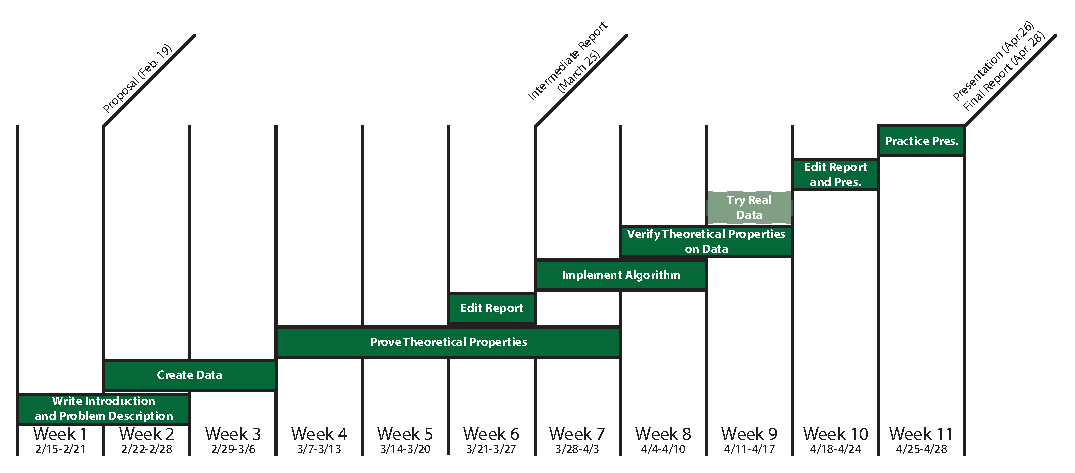
\includegraphics[width=\textwidth]{figures/timeline.eps}
    \caption{Project timeline showing key steps in the project. A solid color border indicates required step while a dotted line border indicates an optional step that will only be completed if there is time.}
    \label{fig:timeline}
\end{figure*}

\subsection{Yinyang K-means}
The proposed work aims to satisfy those three requirements.
It utilizes the triangle inequality in a novel way to keep track of two bounds: the upper bound on the distance from a given point to its assigned cluster center and the lower bound on the distance from the point to any other center.
These two bounds act to reduce the number of distance calculations that need to be performed during the assignment step of K-means.
This is achieved through two kinds of filtering: group/global filtering and local filtering.
Global filtering works to determine if a point needs to be assigned to a different cluster based on the movement of the cluster centers.
If centers change by a large amount, then it is more likely that points need their cluster assignment checked.
Group filtering generalizes the global filtering by initially grouping the clusters into groups before the first iteration of K-means and applying the global filter to those groups.
Local filtering is performed on any groups of cluster centers that make it through the group filter.
Centers that get filtered by the local filter do not have their distances to the data points calculated.

Additionally, a method to optimize the second step of K-means, the center update step, is proposed.
The new method updates the cluster centers by modifying them rather than calculating the average across all points contained in that cluster.



\section{Data}

\begin{table*}[!tb]
\caption{Data Parameters}
\begin{center}
\begin{tabular}{|c||c||c||c|}
\hline
\textbf{Num. of Clusters} & \textbf{Num. of Features} & \textbf{Num. of Samples Per Cluster} & \textbf{Avg. Euclidean Distance of Means} \\
\hline
100 & 100 & 100 & 100 \\
1,000 & 500 & 500 & 500 \\
10,000 & 1,000 & 1,000 & 1,000\\
\hline
\end{tabular}
\end{center}
\label{tab:dataparams}
\end{table*}

The main claim of the authors is the ability to apply the K-means clustering algorithm to data which is large.
Thus, our synthetic dataset should attempt to verify this claim by including large amounts of data.
It will also be interesting to document how the performance changes as the data size grows.
The authors also claim that clustering results of Yinyang K-means is the same as standard K-means.
So we vary the ``difficulty" of clustering the data by varying the average Euclidean distance of the mean of all of the clusters.

There are four primary parameters that we vary in our synthetic dataset.
The first parameter is the number of clusters ($N_C$) where we use 3 different values: 100, 1,000, and 10,000.
The second parameter is the number of features ($N_F$)  where we use 3 different values: 100, 500, and 1,000.
The third parameter is the number of samples per cluster ($N_S$) where we use 3 different values: 100, 500, and 1,000.
The fourth and final parameter is the average mean Euclidean distance parameter ($\mu_\text{euc}$) where we use 3 different values: 100, 500, and 1,000.
There are 81 synthetic datasets that we will run both Yinyang K-means and standard K-means on.
This information is summarized in Table~\ref{tab:dataparams}.


We generate the data as multi-variate Gaussian distributions.
We first generate an $N_C$-sized set of means.
An overview of this process is shown in Figure \ref{fig:meangeneration}.
We want to vary the average distance between clusters so we introduce an average mean Euclidean distance parameter ($\mu_\text{euc}$).
We then use the \texttt{randn} MATLAB function to generate a set of potential means of size $10*N_C$ each with $N_F$ features.
We then sample from the set $N_C$ means and calculate their average Euclidean distance and compare it to $\mu_\text{euc}$.
If it is within the tolerance ($\delta$), we use this as the set of $N_C$ means for a single run.

\begin{figure}[!tb]
    \centering
    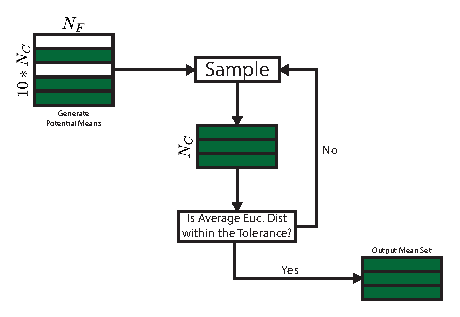
\includegraphics[width=\linewidth]{figures/MeanGeneration.eps}
    \caption{Overview of the mean generation step. A $N_C$-sized set of means is sampled from the $10 * N_C$-sized set of potential means. If the sample has an average Euclidean distance within the tolerance it is selected. If not, a new sample is selected.}
    \label{fig:meangeneration}
\end{figure}

We then generate a random matrix $B$ and then generate a random positive semi-definite matrix $C = B^\text{T} B$ that we use as the covariance.
We do this for each mean in the run.
We use this mean and the covariance as arguments for the \texttt{mvnrnd} MATLAB function to generate the data with $N_S$ samples.


To demonstrate the data generation described above, we used the following parameters: $N_C = 5$, $N_F = 2$, and $N_S = 100$.
Since the data is two dimensional, we can visualize it.
Two examples are shown in Figure \ref{fig:dataexamples}.

\begin{figure}[!tb]
\centering
\subfloat[Example Data 1]{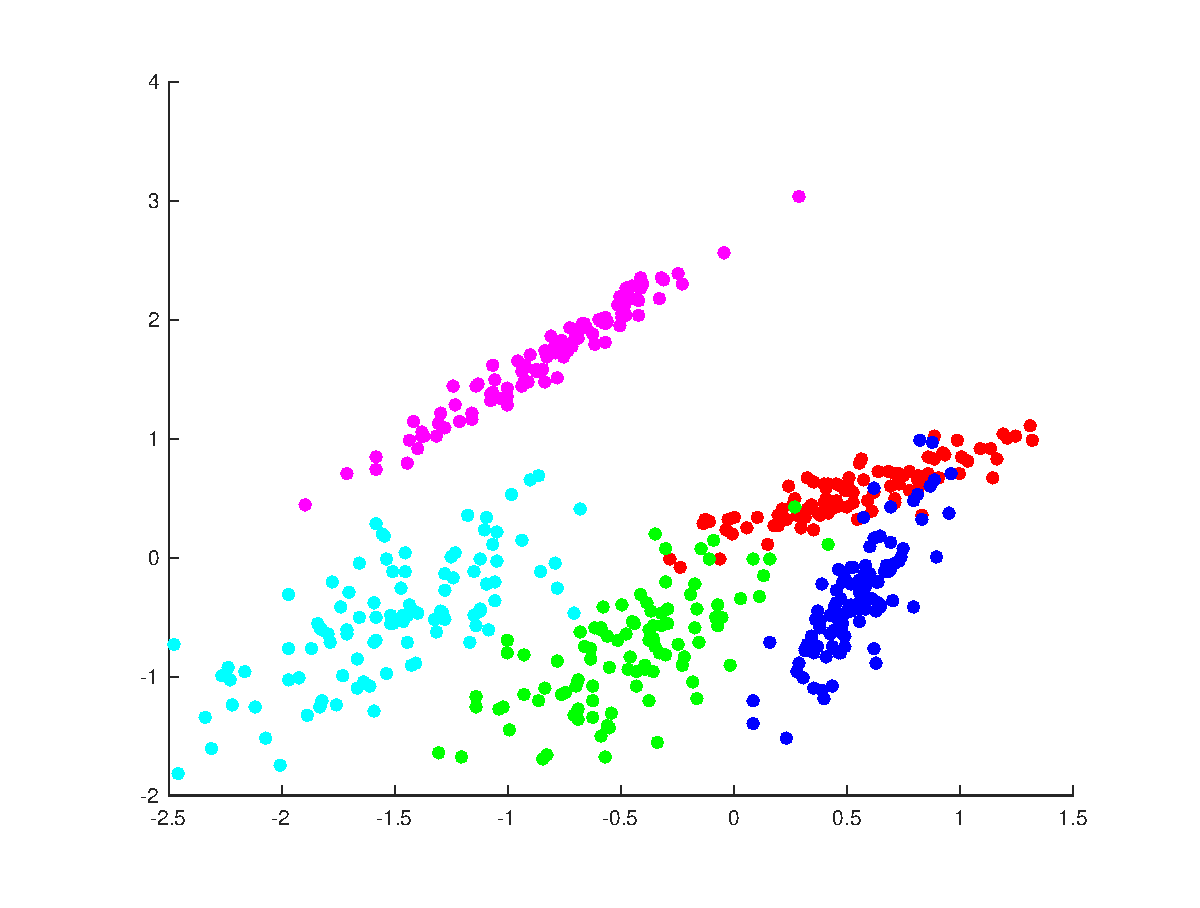
\includegraphics[width = 0.5\linewidth]{figures/RandDataViz.eps}}
~
\subfloat[Example Data 2]{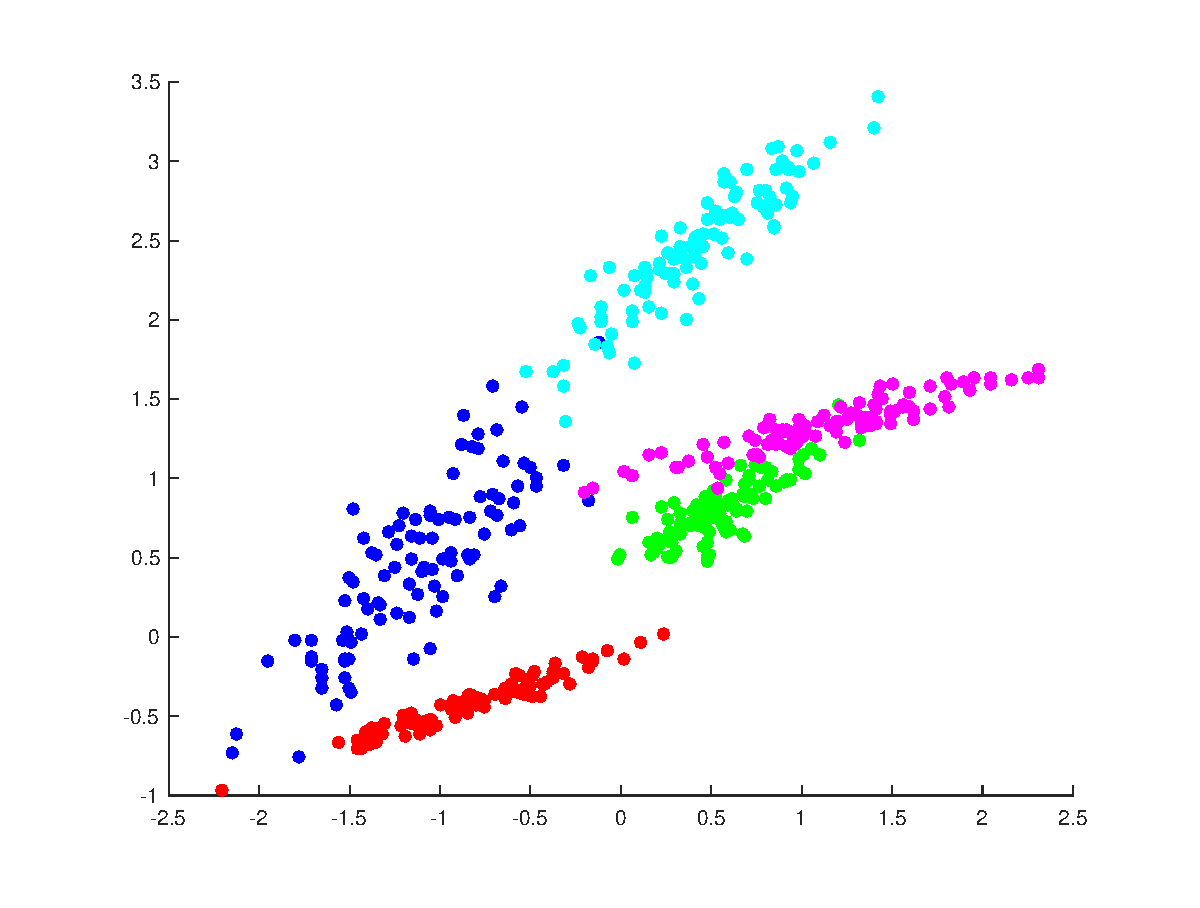
\includegraphics[width = 0.5\linewidth]{figures/RandDataViz2.eps}}
\caption{Examples of generated synthetic data in two dimensions. Each cluster is represented with different colors.}
\label{fig:dataexamples}
\end{figure}

\section{Working Plan}

The theory thrust of the project consists of 3 requirements and a 4th optional task:

\begin{itemize}
\item Show all details of the proof of correctness
\item Implement the algorithm
\item Test algorithm on synthetic dataset to verify theoretical properties
\item \textit{Test algorithm on a real-world dataset}
\end{itemize}

Figure \ref{fig:timeline} shows the overview of our project timeline.
We have completed the introduction and problem description that will be included in the intermediate project report and the final project report.
This document includes a near-final draft of those sections.
We will continue to refine the introduction and problem description as needed.
We have completed the code that generates our synthetic data

The next step is proving the theoretical properties of Yin-yang K-means.
This includes the Global-Filtering Condition and the Local-Filtering Condition.
The Global-Filtering Condition asserts that cluster assignment of a point is only necessary if the cluster centroid changes drastically.
The Local-Filtering Condition allows skipping distance calculations between a point and a centroid if that point is with some set distance to another centroid.
We have made some progress on verifying these theoretical properties, but it is taking somewhat longer than expected.
We will also investigate the authors' claim that Yinyang K-means achieves the same performance as classic K-means with an order of magnitude performance increase.

The last part of the project involves implementing the algorithm on a computer.
Once it is implemented and verified to be correct, we can then test the algorithm on the synthetic data we generated earlier.
The synthetic data has been created in a such a way that the theoretical properties of the algorithm will be tested.
This will tell us that these properties actually hold in practice.
If there is time, we also plan to try the algorithm on a real-world dataset which will hopefully see the same benefits as the synthetic data.

% The following two commands are all you need in the
% initial runs of your .tex file to
% produce the bibliography for the citations in your paper.
\bibliographystyle{abbrv}
\bibliography{yinyang}  % sigproc.bib is the name of the Bibliography in this case
% You must have a proper ".bib" file
%  and remember to run:
% latex bibtex latex latex
% to resolve all references
%
% ACM needs 'a single self-contained file'!
%
%APPENDICES are optional
%\balancecolumns
%\appendix
%Appendix A
%\section{Headings in Appendices}

\end{document}
